\chapter{Implementation of the model\index{Implementation}}
In this chapter we describe two concrete implementations\index{Implementation} of the algebraic model from \chpref{chp:algebraic_model} in \textsf{Haskell}\index{Haskell}. For one of the implementations, we use \textsf{Haskell}'s \texttt{IO} monad and fork local threads for local parallelisation on one computer. For the other one, we use \textsf{Cloud Haskell} to distribute processes into a distributed system and run them in \textsf{Cloud Haskell}'s \texttt{Process} monad.

Ideally, we want the two implementations to be usable interchangeably, however we cannot achieve this at the moment. When using the implementation based on the \textsf{Cloud Haskell} \texttt{Process} monad, we need to require additional properties of the data types that are transmitted over the network as arguments and results of processes. Furthermore, in order to run code remotely, the code has to be known on the remote node since ghc\footnote{The Glasgow Haskell Compiler, c.f. \url{https://www.haskell.org/ghc/}.} doesn't support serialising and transmitting functions over the network \cite{Epstein:2011:THC:2034675.2034690}. To solve this problem, a trick is used that requires us to change the model of basic processes slightly.

%We start off with the definition of the data structure and then take a closer look at the implementation of the interpreter\index{Interpreter} that takes care of the distribution of process structures in a distributed system\index{Distributed system}. We conclude this chapter with an examples that illustrates how to use our process calculus to solve problems.

\section{Implementation in the IO monad}
\label{chp:local}
In the implementation for local parallelisation on only one computer, we make use of \textsf{Haskell}'s \texttt{IO} monad and the \texttt{Control.Concurrent} package. Basic processes are represented as computations in the \texttt{IO} monad. Parallelisation is achieved by running processes that have been modelled for parallel execution in lightweight threads using \texttt{forkIO}, synchronisation is done using \texttt{MVars}.

We do not discuss the basic principles of the \texttt{IO} monad here, an introduction can be found in standard \textsf{Haskell} literature such as \cite{Hutton} or \cite{Bird}. However, the fact that we use the \texttt{IO} monad has immediate consequences: we \textbf{can not} force processes to be free of side-effects\index{Side-effect}. Actually processes can perform any kind of action they like, including reading from or writing to the file system, executing queries on databases or accessing web resources. As we will see later, this motivates us not to implement an automated process optimiser.

\subsection{Data model}
\label{chp:local_model}
Our data model resembles the structure of the algebraic model\index{Algebraic!model} given in \chpref{chp:algebraic_model}. We aim to prevent the creation of erroneous processes and check for their validity at compile time. To achieve this, we employ a generalised algebraic data type\index{Generalised algebraic data type} and leverage the power of \textsf{Haskell}'s type system. 

As mention in the introduction of this chapter, we run basic processes as computations in the \texttt{IO} monad. For later, we also introduce how we represent predicates.
\begin{lstlisting}[language=Haskell,caption=Representation of basic processes as computations in the \texttt{IO} monad.,label=fig:local_computation,numbers=left,frame=bt]
type Predicate    a = a	 -> Bool
type BasicProcess b = IO b
\end{lstlisting}

Our data type for processes involves two type parameters\index{Type!parameter}, \texttt{a} and \texttt{b}. They reflect the types of the process' argument\index{Argument}\index{Type!argument} and result\index{Result}\index{Type!result} values where \texttt{a} is the type of the argument and \texttt{b} is the type of the result.
\begin{lstlisting}[language=Haskell,caption=Data type for the representation of processes.,label=fig:local_datatypes,numbers=left,frame=bt,firstnumber=2]
data Process a b where
\end{lstlisting}

We have two data constructors for wrapping values of type \texttt{BasicProcess}\index{Process!basic} into a \texttt{Process}, i.e. \texttt{Const} and \texttt{Simple}. In principle, it is possible to use a \texttt{BasicProcess} of arbitrary complexity to create a \texttt{Process}, but regarding possible transformations based on the laws introduced in \chpref{chp:laws}, we require them to be free of side-effects. If they incorporate side-effects, their semantics can not be guaranteed to remain unchanged after transformation\footnote{Idempotent\index{Idempotence} actions however, \textit{should} not alter processes' semantics, regardless of transformations that may be performed.} into a different representation. A process' behaviour should be fully determined by its input and repeated execution of the same process with the same input should always yield the same output.

The \texttt{Const}\index{Data constuctor!Const} data constructor takes a value of type \texttt{BasicProcess} and always produces the same output when executed\footnote{Given the \texttt{BasicProcess} behaves like a function in the mathematical sense.}.
\begin{lstlisting}[language=Haskell,caption=Signature of the \texttt{Const} data constructor.,numbers=left,frame=bt,firstnumber=3]
Const :: BasicProcess b
      -> Process a b
\end{lstlisting}

\texttt{Simple}\index{Data constructor!Simple} takes a parametrised \texttt{BasicProcess}\index{Process!basic} of type \texttt{a $\to$ BasicProcess b} that behaves like a 1-ary function.
\begin{lstlisting}[language=Haskell,caption=Signature of the \texttt{Simple} data constructor.,numbers=left,frame=bt,firstnumber=5]
Simple :: (a -> BasicProcess b)
       -> Process a b
\end{lstlisting}

\texttt{Const} and \texttt{Simple} are data constructors just for wrapping basic processes into the \texttt{Process} data type. Essentially they represent what we calles atomic processes in \chpref{chp:algebraic_model}. All other data constructors\index{Constructor} operate on existing processes and resemble the algebraic operations from \chpref{chp:algebraic_model}, such as choice, parallel composition, sequential composition and \textsc{Kleene} star. However, as we will see, some of the data constructors are more general and thus more expressive and flexible than the operators presented in \chpref{chp:algebraic_model}.

Regardless of how complex a \texttt{BasicProcess} wrapped into a \texttt{Process} of type \texttt{Const} or \texttt{Simple} actually is, we consider them to be atomic for the following discussions since they do not involve process combinators.

The \texttt{Choice}\index{Data constructor!Choice} data constructor is used to build a process that makes a choice between two processes and represents the choice operator $\choice$. Unlike in the algebraic model from \chpref{chp:algebraic_model}, this choice is not made non-deterministically by an oracle\index{Oracle}, but based on a predicate\index{Predicate}. The introduced predicate makes sure the behaviour of a process that involves the \texttt{Choice} combinator is always determined and exactly one result is produced. \texttt{Choice} takes a value of type \texttt{c}, a function of type \texttt{a $\to$ c $\to$ d}, a predicate \texttt{Predicate d} and two processes of type \texttt{Process a b}.
\begin{lstlisting}[language=Haskell,caption=Signature of the \texttt{Choice} data constructor.,numbers=left,frame=bt,firstnumber=7]
Choice :: c
       -> (a -> c -> d)
       -> Predicate d
       -> Process a b
       -> Process a b
       -> Process a b
\end{lstlisting}

The \texttt{Sequence}\index{Data constructor!Sequence} data constructor takes two processes and composes them sequentially, it represents the sequence operator $\sequence$. Similar to conventional function composition, the result type of the first process and the input type of the second process must coincide.
\begin{lstlisting}[language=Haskell,caption=Signature of the \texttt{Seqeuence} data constructor.,numbers=left,frame=bt,firstnumber=13]
Sequence :: Process a c
         -> Process c b
         -> Process a b
\end{lstlisting}

With the \texttt{Parallel}\index{Data constructor!Parallel} data constructor, we can create a \texttt{Process} that runs two processes in parallel. As the signature of \texttt{Parallel} shows, our model for parallel composition of processes is more general than the one introduced in \chpref{chp:algebraic_model}. Where in the algebraic model, we can only combine two processes with the parallel combinator $\parallel$ iff they have the same type signature and their result type forms a semigroup\index{Semigroup} with a commutative binary operation, we can use arbitrary processes for parallel composition in our implementation. However, they need to accept the same input type. \texttt{Parallel} takes two processes, with types \texttt{Process a c} and \texttt{Process a d}, that are to be composed in a parallel way. In addition to that, it takes a third process of type \texttt{Process (c, d) b}, and uses it to combine the results of the other two processes after they have finished execution and returned their results. Note that using an explicit process to combine the results is exactly what enables us to compose processes of different types in parallel. At the same time we eliminate the required structure of a semigroup on their result type.
\begin{lstlisting}[language=Haskell,caption=Signature of the \texttt{Parallel} data constructor.,numbers=left,frame=bt,firstnumber=16]
Parallel :: Process a c
         -> Process a d
         -> Process (c, d) b
         -> Process a b
\end{lstlisting}

\texttt{Multilel}\index{Data constructor!Multilel} represents the generalisation of parallel composition of two processes to parallel composition of an arbitrary number of processes. It takes a list of processes of type \texttt{Process a c}, a value of type \texttt{b} and a process of type \texttt{Process (b, [c]) b}. The list of processes contains the processes that should be composed in parallel, the additional process together with the value of type \texttt{b} is used to fold the results of the processes together.
\begin{lstlisting}[language=Haskell,caption=Signature of the \texttt{Multilel} data constructor.,numbers=left,frame=bt,firstnumber=20]
Multilel :: [Process a c]
         -> b
         -> Process (b, [c]) b
         -> Process a b
\end{lstlisting}

With the \texttt{Loop}\index{Data constructor!Loop} data constructor, we can wrap a process for repeated execution, resembling the \textsc{Kleene} star $\repetition$. However, we provide a much more sophisticated and more general version than the \texttt{Kleene} star does. First, \texttt{Loop} takes a value of type \texttt{b}, which serves as a default output value in case the loop is executed exactly zero times. In imperative programming, this corresponds to the implicitly unchanged global state of the program. Then it takes a value of type \texttt{c}, a predicate \texttt{Predicate c} and a function of type \texttt{a $\to$ c $\to$ c}. The combination of these three control the termination of the \texttt{Loop}'s execution. The function of type \texttt{b $\to$ a} is used to convert the result of the process of type \texttt{Process a b} back to a value of type \texttt{a}, so it can be fed into the next execution of the \texttt{Loop}. Note that a \texttt{Loop} process does not necessarily behave like the identity process $Id$ if it runs zero times. Responsible for this is the explicit default value of type \texttt{b} which is returned in this case.
\begin{lstlisting}[language=Haskell,caption=Signature of the \texttt{Loop} data constructor.,numbers=left,frame=bt,firstnumber=34]
Loop :: b
     -> c
     -> Predicate d
     -> (b -> a)
     -> (a -> c -> d)
     -> Process a b
     -> Process a b
\end{lstlisting}


\subsection{Process interpreter}
In this chapter we discuss how the \texttt{Process} interpreter works in detail by taking a look at the implementation.

\texttt{Process}es can be run using the \texttt{runProcess} function. It takes a value of type \texttt{Process a b} and an argument of type \texttt{a} for the process. It runs in the \texttt{IO} monad and produces a result of type \texttt{b}.
\begin{lstlisting}[language=Haskell,caption=Signature of the process interpreter.,label=lst:local_runprocess_signature,numbers=left,frame=bt]
runProcess :: Process a b -> a -> IO b
\end{lstlisting}

The interpretation of a \texttt{Const}\index{Process interpreter!Const} process is straightforward. Since \texttt{Const} processes don't take an argument, we simply discard it and run the wrapped basic process \texttt{bp}, as shown in \lstref{lst:local_runprocess_const}.
\begin{lstlisting}[language=Haskell,caption=Implementation of the interpreter of \texttt{Const} processes.,label=lst:local_runprocess_const,numbers=left,frame=bt,firstnumber=2]
runProcess (Const bp) _ =
  bp
\end{lstlisting}

The interpretation of \texttt{Simple}\index{Process interpreter!Simple} processes is similarly easy. We simply take the wrapped basic process \texttt{bp} and pass the argument \texttt{x} to it, as \lstref{lst:local_runprocess_simple} shows.
\begin{lstlisting}[language=Haskell,caption=Implementation of the interpreter for \texttt{Simple} processes.,label=lst:local_runprocess_simple,numbers=left,frame=bt,firstnumber=4]
runProcess (Simple bp) x =
  bp x
\end{lstlisting}

Unlike in the algebraic model\index{Algebraic!model}, specifically \defref{def:static_choice} and \defref{def:sem_choice}, a \texttt{Choice} process does not introduce non-determinism\index{Non-determinism}. Earlier we used an optimistic oracle\index{Oracle} to make the choice between two processes, but didn't have any control over the oracle's behaviour, thus introducing non-determinism. In order to get rid of the non-determinism we replace the non-deterministic oracle with a deterministic predicate\index{Predicate} \texttt{pr} of type \texttt{Predicate d} that makes the choice between processes, as shown in \lstref{lst:local_runprocess_choice}. The predicate's choice is based on a value \texttt{c} and the arguments for the process \texttt{x} of type \texttt{a}. These two values are combined using the function \texttt{acd :: a $\to$ c $\to$ d} and the result is presented to the predicate \texttt{pr}. If \texttt{pr (acd x c)} holds, the first process \texttt{p1} is selected for execution and the second process \texttt{p2} otherwise. Note that we have eliminated one of the two places where there was non-determinism introduced in the algebraic model.
\index{Process interpreter!Choice}
\begin{lstlisting}[language=Haskell,caption=Implementation of the interpreter for \texttt{Choice} processes.,label=lst:local_runprocess_choice,numbers=left,frame=bt,firstnumber=6]
runProcess (Choice c acd pr p1 p2) x =
  runProcess (if pr (acd x c) then p1 else p2) x
\end{lstlisting}

For the interpretation of a \texttt{Sequence}\index{Process interpreter!Sequence} process, we have to run the first process \texttt{p1} on the argument \texttt{x} first by making use of the interpreter function \texttt{runProcess}. Then, using the result from \texttt{p1}, we run the second process \texttt{p2}. The implementation of this is straightforward, using \texttt{IO}'s bind operator \texttt{>}\texttt{>=}, as shown in \lstref{lst:local_runprocess_sequence}.
\begin{lstlisting}[language=Haskell,caption=Implementation of the interpreter for \texttt{Sequence} processes.,label=lst:local_runprocess_sequence,numbers=left,frame=bt,firstnumber=8]
runProcess (Sequence p1 p2) x =
  runProcess p1 x >>= runProcess p2
\end{lstlisting}

In the implementation of the interpreter function \texttt{runProcess} so far, there has been no parallelism introduced. However, the purpose of our process calculus is to make parallel programming easy and intuitive. Hence, we need a mechanism to introduce parallelism. This is done with the \texttt{Parallel} and \texttt{Multilel} combinators for processes. Whereas \texttt{Parallel} allows for parallel composition of two \texttt{Process}es with arbitrary types, \texttt{Multilel} allows for parallel composition of arbitrary many processes of a common type.

So far, we could simply perform the interpretation of processes in the interpreter thread because we only had one program flow. This changes in the case of the \texttt{Parallel} and \texttt{Multilel} processes where we explicitly have two or more program flows. That means we have to fork at least one more thread for parallel interpretation of the processes. We introduce an auxiliary interpreter function \texttt{runProcessHelper} for this. It takes a process of type \texttt{Process a b}, an argument of type \texttt{a} for the process and an \texttt{MVar b} that is used to communicate the result back to the caller. \texttt{runProcessHelper} runs in the \texttt{IO} monad and its behaviour is fairly simple: it runs the process interpreter \texttt{runProcess} for the submitted process by passing process \texttt{p} and argument \texttt{x} to it and saving the obtained result in \texttt{mvar}, then it terminates. The implementation of \texttt{runProcessHelper} can be found in \lstref{lst:local_runprocesshelper}.
\begin{lstlisting}[language=Haskell,caption=Auxiliary process for the interpretation of \texttt{Parallel} and \texttt{Multilel} processes.,label=lst:local_runprocesshelper,numbers=left,frame=bt,firstnumber=10]
runProcessHelper :: Process a b -> a -> MVar b -> IO ()
runProcessHelper p x mvar = putMVar mvar =<< runProcess p x
\end{lstlisting}

A \texttt{Parallel}\index{Process interpreter!Parallel} process incorporates exactly two processes, \texttt{p1} and \texttt{p2}, that should be run in parallel as well as a combinator process, \texttt{combinator}, that is intended to be used to combine the results from \texttt{p1} and \texttt{p2}. To accomplish parallel execution of \texttt{p1} and \texttt{p2}, we create a new empty \texttt{MVar} and use \texttt{forkIO} to fork a new thread which we run \texttt{runProcessHelper} in. Together with its argument \texttt{x} and the \texttt{mvar}, Process \texttt{p1} is passed to the new thread for interpretation. At the same time, we start interpretation of process \texttt{p2} in the current interpreter thread. After the interpretation of \texttt{p2} has finished, we retrieve the result of the interpretation of \texttt{p1} from \texttt{mvar}. If execution of \texttt{p1} hasn't finished yet, this operation blocks until this is the case and the result has been saved to \texttt{mvar}. Once we have the results of both \texttt{p1} and \texttt{p2}, we start the interpretation of \texttt{combinator} that combines these results into one value. Again, the combinator process is why we can combine processes of arbitrary types in parallel, in contrast to what we saw in the algebraic model in \chpref{chp:algebraic_model}.
\begin{lstlisting}[language=Haskell,caption=Implementation of the interpreter for \texttt{Parallel} processes.,numbers=left,frame=bt,label=lst:local_runprocess_parallel,firstnumber=12]
runProcess (Parallel p1 p2 combinator) x = do
  mvar <- newEmptyMVar
  _ <- forkIO $ runProcessHelper p1 x mvar
  r2 <- runProcess p2 x
  r1 <- takeMVar mvar
  runProcess combinator (r1, r2)
\end{lstlisting}

The interpretation of a \texttt{Multilel}\index{Process interpreter!Multilel} process follows the same principles as the interpretation of a \texttt{Parallel} process. The difference only lies in that we have to deal with a list of processes that should be run in parallel instead of exactly two. This has some consequences: we require all of these processes to have the same type, otherwise we would end up with $n-1$ combinator processes for the combination of the results from $n$ processes. By requiring the same type for every process and thus, the same result type, we can reduce the requirement for combinator processes to only one process, namely \texttt{fold}, and one value, namely \texttt{ib}, as can be seen in \lstref{lst:local_runprocess_multilel}. As the name \texttt{fold} suggests, this process behaves like a fold: it takes a pair that contains the initial fold value \texttt{ib} and a sequence of values, namely \texttt{ress}, that should be folded together into one result value. For parallel execution of all the processes in \texttt{ps}, we create a new empty \texttt{MVar} for each of them and start a \texttt{runProcessHelper} in a new thread for each of them, supplying one of the \texttt{mvars} per thread. Then we wait for all of the processes to finish execution by reading their results from the \texttt{mvars}. Should there be even a single process that hasn't finished execution, the according \texttt{MVar} blocks the reading action until a value has been saved into it. Finally, the \texttt{fold} process is run, folding the results together and returning a single result.
\begin{lstlisting}[language=Haskell,caption=Implementation of the interpreter for \texttt{Multilel} processes.,label=lst:local_runprocess_multilel,numbers=left,frame=bt,firstnumber=18]
runProcess (Multilel ps ib fold) x = do
  mvars <- forM ps $ const newEmptyMVar
  mapM_ (\(p, m) -> forkIO $ runProcessHelper p x m) (ps `zip` mvars)
  ress  <- forM mvars takeMVar
  runProcess fold (ib, ress)
\end{lstlisting}

Finally, there is the \texttt{Loop}\index{Process interpreter!Loop} process that is used to resemble the semantics of the \textsc{Kleene} star, i.e. repeated execution of a process. However, we're altering the semantics slightly: as we did for the \texttt{Choice} process, we want to eliminate non-determinism here as well and end up with a determined number of repetitions of a process. To do so, we replace the oracle\index{Oracle} that selects how often the process should be run with a predicate\index{Predicate} that decides whether execution should terminate or continue. The structure of the interpreter function for a \texttt{Loop} process reminds of a \texttt{while} loop in imperative programming, however its behaviour in case of zero time execution is explicitly defined. A \texttt{Loop} process contains six values: \texttt{ib} of type \texttt{b}, \texttt{ic} of type \texttt{c}, a predicate\index{Predicate} \texttt{pred} of type \texttt{Predicate c}, a function \texttt{ba} of type \texttt{b $\to$ a}, a function \texttt{acc} of type \texttt{a $\to$ c $\to$ c} and a process \texttt{p} of type \texttt{Process a b}. The value \texttt{ib} defines the result value of the \texttt{Loop} process in case it is executed zero times. In imperative programming, this is the implicit program state that is unaltered whenever a loop executed zero times. In order to decide whether the process wrapped into the \texttt{Loop} should be executed, the previously mentioned predicate \texttt{pred} is evaluated. It takes its decision based on an initial value \texttt{ic} and the argument for the process \texttt{x}, combined together by \texttt{acc}. If the predicate holds, the process \texttt{p} is executed once and its result is bound to the name \texttt{x'}. Then, a new \texttt{Loop} process is created and the \texttt{runProcess} interpreter is called tail-recursively on it. The argument for the new \texttt{Loop} process is given by \texttt{x'}, converted from type \texttt{b} to a value of the correct type \texttt{a} by function \texttt{ba}. Remember that in \defref{def:static_kleene}, the definition of the static semantics of the \textsc{Kleene} star, we had required that a process that should be run repeatedly, needs to have the same input and output type. However, by employing a function, namely \texttt{ba}, that converts the result of a process back to the type of its argument, we can get rid of this requirement. Once again, the semantics of the \texttt{Loop} process in our process calculus is more general than the one of the \textsc{Kleene} star from the algebraic model.
\begin{lstlisting}[language=Haskell,caption=Implementation of the interpreter for \texttt{Loop} processes.,numbers=left,frame=bt,firstnumber=23]
runProcess (Loop ib ic pr ba acc p) x = do
  if pr (acc x ic) then do
    x' <- runProcess p x
    runProcess (Loop x' (acc x ic) pr ba acc p) (ba x')
  else
    return ib
\end{lstlisting}


\section{Implementation in the Cloud Haskell Process monad}
\label{chp:distributed}
In the implementation for distributed parallelisation of process interpretation, we use \textsf{Cloud Haskell}'s \texttt{Process} monad. The involvement of network communication requires that we provide instances of specific type classes for the types that are to be sent over network. Furthermore, we need to adapt our representation of basic processes and some process types to the specifics of \textsf{Cloud Haskell}. 

\subsection{\index{Cloud Haskell}Cloud Haskell}
\label{chp:cloud_haskell}
\textsf{Cloud Haskell} \cite{Epstein:2011:THC:2034675.2034690} is a domain specific language for distributed programming in Haskell. It is highly inspired by Erlang\index{Erlang} and its message passing\index{Message passing} mechanism for communication between processes. Like it is typical for \textsf{Haskell}, there is no implicitly shared memory involved.

A \textsf{Cloud Haskell} process is essentially a function\index{Function} that is evaluated in the \texttt{Process} monad\index{Monad} and can be spawned on a local\index{Node!local} or remote\index{Node!remote} node. Processes can send messages to other processes if they have knowledge about their process identifier, which serves as an address. The \texttt{Process} monad builds on top of the \texttt{IO} monad and thus, as mentioned in \chpref{chp:local}, we can not force processes to be free of side-effects.

While Erlang\index{Erlang} uses atoms as tags for messages, \textsf{Cloud Haskell} uses data types that need to have an instance of \texttt{Serializable}. \texttt{Serializable} itself is only a combination of both \texttt{Binary} and \texttt{Typeable}. \texttt{Binary} is neccessary to serialise a message into a \texttt{ByteString}, \texttt{Typeable} is used to identify the type of a value. This way, serialisation\index{Serialisation} is made explicit, in contrast to Erlang where it is implicit \cite{Epstein:2011:THC:2034675.2034690}.

In \textsf{Haskell}, functions can only be executed, composed and passed as arguments, they cannot be serialised. However, this is be necessary in order to send a function to a remote\index{Node!remote} node and execute it there. \textsf{Cloud Haskell} avoids this problem by using a table of static code pointers, i.e. fully qualified top level names of functions that are known at compile time, to refer to functions by a name. For remote execution, a function's name is put into a \texttt{Closure}\index{Closure}, together with its serialised environment\index{Environment}, i.e. its argument, and sent to a remote node where it is deserialised and executed. A \texttt{Closure} is nothing more than just mentioned: a function (name) together with its argument \cite{Epstein:2011:THC:2034675.2034690} and can be created using \textsf{Cloud Haskell}'s function \texttt{mkClosure} and \textsf{Template Haskell}. \texttt{mkClosure} takes the top level name of a function and returns a closure generator. The function supplied to \texttt{mkClosure} needs to be of 1-ary type \texttt{a $\to$ Process b} and return a \textsf{Cloud Haskell} process. For a function \texttt{f} of type \texttt{a $\to$ Process b}, the type of \texttt{\$(mkClosure 'f)} resolves to \texttt{a $\to$ Closure (Process b)}, i.e. it is a closure generator that generates a closure when supplied with a value of type \texttt{a}.

After a \texttt{Closure} has been executed, the result is serialised and sent back to the caller. However, in some cases, the type system cannot infer the serialisability of the result type and therefore additional information needs to be provided\footnote{Specifically, the problem is that the type constructors can be constrained with required type class instances for parameters. On deconstruction, this information is not available and therefore needs to be added explicitly again.}. For a type \texttt{a}, serialisation information can be provided with a value of type \texttt{Static (SerializableDict a)}. Essentially this is only an explicit type tag that enables the selection of the correct serialisation function for type \texttt{a}.

\subsection{Data model}
\label{chp:distributed_model}
The data model for the representation of processes in the \textsf{Cloud Haskell} \texttt{Process} monad is essentially the same as what we saw in \chpref{chp:local_model}. Predicates are still functions that return a \textsc{Bool}ean value and basic processes are computations in the \textsf{Cloud Haskell} \texttt{Process} monad. In the following \texttt{CH} is the name for the qualified import of \texttt{Control.Distributed.Process}.
\begin{lstlisting}[language=Haskell,caption=Representation of basic processes as computations in the \texttt{Process} monad.,numbers=left,frame=bt]
import qualified Control.Distributed.Process as CH

type BasicProcess b = CH.Process b
\end{lstlisting}

The signature of our representation of processes remains unchanged, only the data constructors need to be changed slightly.
\begin{lstlisting}[language=Haskell,caption=Data type for the representation of processes.,label=fig:distributed_datatypes,numbers=left,frame=bt,firstnumber=4]
data Process a b where
\end{lstlisting}

The wrappers for basic processes, i.e. \texttt{Const} and \texttt{Simple} reflect the necessary adaptations that come with \textsf{Cloud Haskell}: they constrain the result type of the wrapped basic process to be an instance of the type class \texttt{Serializable} and require a static \texttt{SerializableDict} for the same type. As mentioned in \chpref{chp:cloud_haskell}, this is necessary so remotely\footnote{This is true for locally spawned processes as well, as we can conceptually not distinguish between them: \textsf{Cloud Haskell} transparently takes care of that we can use both local and remote processes in the same way. Technically, however, we could inspect the process identifier and tell if the respective process is running on the same or a different node.} spawned processes know how to serialise their result and send it back to the caller. Instead of a value of type \texttt{BasicProcess} as before, \texttt{Const} takes a closure that contains a basic process. Similarly, \texttt{Simple} takes a closure generator, i.e. a function that, supplied with a value of the appropriate type, generates a closure. %ToDo
\begin{lstlisting}[language=Haskell,caption=Signature of the \texttt{Const} and \texttt{Simple} data constructors.,numbers=left,frame=bt,firstnumber=5]
Const  :: (Serializable b) 
       => CH.Static (SerializableDict b)
       -> CH.Closure (BasicProcess b)
       -> Process a b

Simple :: (Serializable b)
       => CH.Static (SerializableDict b)
       -> (a -> CH.Closure (BasicProcess b))
       -> Process a b
\end{lstlisting}

We extend our model for processes and add the \texttt{Local}\index{Data constructor!Local} data constructor. \texttt{Local} is a simple decorator\index{Decorator} \cite{Gamma:1995:DPE:186897}, with the purpose to give an indication to the process interpreter that the wrapped process should be executed locally. Typically, the reason for this arises from the expectation that serialising a closure, sending it to a remote node, executing it there and obtaining the result is more expensive\footnote{Expensive in terms of the necessary amount of time to run the process.} than executing the respective process locally. Since there is no general approach to estimate the necessary amount of time to run a process, we decide to equip the user with a tool to force local execution of a process and burden him with the obligation to make appropriate use of it.
\begin{lstlisting}[language=Haskell,caption=Signature of the additional \texttt{Local} data constructor.,numbers=left,frame=bt,firstnumber=14]
Local :: Process a b
      -> Process a b
\end{lstlisting}

The signature of the rest of the data constructors, i.e. \texttt{Sequence}, \texttt{Parallel}, \texttt{Multilel} and \texttt{Loop}, remain unchanged.

\subsection{Architecture of the infrastructure\index{Architecture}}
\label{chp:infrastructure}
For the interpretation of process structures in a distributed system, we need some kind of infrastructure and management of involved nodes, so we can delegate process execution to them. In this chapter, we describe the architecture and functioning of our system.
\begin{figure}[h!]
  \centering
  \begin{tikzpicture} [every node/.style={fill=black, circle, inner sep = 2pt}]
    \pgftext{
      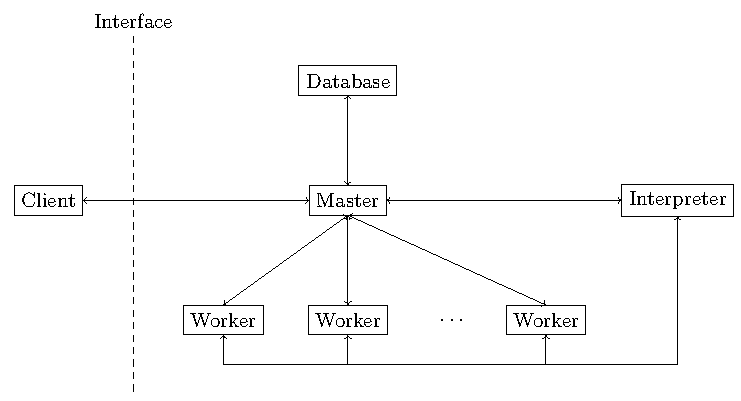
\includegraphics[width=\textwidth]{img/architecture.pdf}
    }
    \node at (-4.25, 0.25) {\tiny \color{white} 1};
    \node at (-3.75, 0.25) {\tiny \color{white} 2};
    \node at ( 1.50, 0.25) {\tiny \color{white} 3};
    \node at (-0.10, 1.75) {\tiny \color{white} 4};
    \node at (-3.25, 0.25) {\tiny \color{white} 5};
    \node at ( 2.00, 0.25) {\tiny \color{white} 6};
    \node at (-0.10, 1.25) {\tiny \color{white} 7};
    \node at (-2.75, 0.25) {\tiny \color{white} 8};
    \node at (-0.10, 0.75) {\tiny \color{white} 9};
    \node at (-2.30,-1.25) {\tiny \color{white} 10};
    \node at (-0.80,-1.25) {\tiny \color{white} 10};
    \node at ( 2.50,-1.25) {\tiny \color{white} 10};
    \node at ( 1.00,-3.60) {\tiny \color{white} 11};
    \node at ( 6.10, 0.65) {\tiny \color{white} 12};
    \node at ( 2.50, 0.30) {\tiny \color{white} 13};
    \node at ( 3.10, 0.30) {\tiny \color{white} 14};
    \node at ( 3.70, 0.30) {\tiny \color{white} 15};
  \end{tikzpicture}
  \caption{Architecture of the infrastructure }
  \label{fig:architecture}
\end{figure}

The architecture of our system's infrastructure is intentionally kept simple as shown in \figref{fig:architecture}. It involves a designated \textbf{master}\index{Node!master} node and a collection of \textbf{worker}\index{Node!worker} nodes. In addition to that, we need an interface\index{Interface} through which we can insert processes into the system. The easiest way to do so is a command line interface, however, a web interface would be much more convenient and easier to use. We employ Yesod\footnote{Yesod is a Haskell web framework. More information about Yesod can be found at \url{http://www.yesodweb.com/} and \url{https://github.com/yesodweb/yesod}}\index{Yesod} to build a RESTful\index{REST} web interface.

When a client\index{Client} wants to submit a request\index{Request} \figannotation{1}, it has to make use of the web interface and supply a JSON\footnote{JavaScript Object Notation \url{http://www.json.org/}}\index{JSON} document in an appropriate format. In a productive environment, there would be a parser that reads a submitted JSON document, generates a corresponding process structure from its content and passes it on to the process interpreter if the document is valid. For simplicity, we assume for now that a request equals a valid process description and can be interpreted.

The master\index{Node!master} node is responsible for handling client\index{Client} requests, logging information related to the received requests and managing connected nodes. When a request is received \figannotation{2}, the master spawns a new \textsf{Cloud Haskell} \texttt{Process} that runs the \textsc{Hive} process interpreter\index{Interpreter} and passes the request to the new process where it is interpreted \figannotation{3}. At the same time, the master assigns a ticket id to the request, logs the request together with its id to a database\footnote{For this purpose, we make use the \texttt{acid-state} library. \texttt{acid-state} allows to save Haskell values into a file-based database if their type has an instance of \texttt{SafeCopy}. Further information on \texttt{acid-state} can be found at \url{http://acid-state.seize.it/} and \url{https://github.com/acid-state/acid-state}} \figannotation{4} and reports the ticket id to the client \figannotation{5}. When the interpreter finishes interpreting the process structure from the request, it reports the result to the master \figannotation{6}. The master then updates the database \figannotation{7} by logging the result to the database and linking it to the according id. At any time, a client can try to retrieve the result to its request by supplying the request's ticket id to the master through the interface \figannotation{8}. The master then tries to read the result from the database \figannotation{9}, but only replies to the client's satisfaction after the interpretation of its request has been finished and logged to the database.

Worker nodes\index{Node!worker} are kept very simple. When started and supplied with the master's address, they report their availability to the master \figannotation{10} and wait for further instruction.

The \textsc{Hive} process interpreter\index{Interpreter}, which we discuss in full detail in \chpref{chp:interpreter}, is run in a new process by the master for every client request\index{Request} that is received. The interpreter inspects the structure of the received request, transforms it into a \textsc{Hive} process structure and distributes the incorporated sub-processes\index{Sub-process} to worker\index{Node!worker} nodes \figannotation{11} or executes them locally \figannotation{12} if they have been marked for local execution using the \texttt{Local} wrapper. For every basic sub-process, the interpreter asks the master for a worker node \figannotation{13} where it can run the sub-process. For such a request, the master fetches a worker node from a FIFO queue and returns it to the interpreter \figannotation{14}. After a sub-process has finished execution on a worker node, the interpreter returns the respective worker node to the master \figannotation{15} for future allocation to other interpreters. It would very well be possible to employ a more sophisticated scheduling\index{Scheduling} algorithm, but the combination of a FIFO\index{FIFO} queue and a work stealing\index{Work stealing} \cite{} alike behaviour of the process interpreter is fairly efficient and easy to implement. At this time, our primary goal is not to achieve the best possible load balancing or employ the most efficient technique for queueing worker nodes, however this leaves room for future improvement.


\subsection{Process interpreter\index{Process interpreter}\index{Interpreter}}
\label{chp:interpreter}
With the involvement of a distributed system, we need to change the implementation of the process interpreter. Where there was only local parallelisation in the \texttt{IO} monad involved before, we have to adapt process interpretation to the specifics of the \textsf{Cloud Haskell} \texttt{Process} monad. This particularly involves remote execution of processes.

When the master\index{Node!master} node receives a client\index{Client} request\index{Request}, it spawns a process interpreter on its local node and passes the process structure from the request to the interpreter. The interpreter then inspects the process structure and distributes the incorporated sub-processes\index{Sub-process} to connected worker nodes accordingly. To do so, the interpreter asks the master node for an available worker node for every sub-process that has to be executed\footnote{Except for processes wrapped into a \texttt{Local} process, of course.}. We represent the master\index{Node!master} node by a \texttt{ProcessId} that is wrapped into a value of type \texttt{Master}.
\begin{lstlisting}[language=Haskell,caption=Data type for the address of a master node.,numbers=left,frame=bt]
newtype Master = Master ProcessId
\end{lstlisting}

We have to adapt the signature of \texttt{runProcess} and introduce an additional parameter, as shown in \lstref{lst:interpreter_signature}. As before, \texttt{runProcess} takes a process of type \texttt{Process a b}, an argument for the process of type \texttt{a} and returns a value of type \texttt{b}. Furthermore, for process distribution, \texttt{runProcess} requires a value of type \texttt{Master}, so it can request worker nodes to run processes on.
\begin{lstlisting}[language=Haskell,caption=Signature of the process interpreter.,label=lst:interpreter_signature,numbers=left,frame=bt,firstnumber=2]
runProcess :: Master -> Process a b -> a -> CH.Process b
\end{lstlisting}

For the interpretation of a \texttt{Const}\index{Process interpreter!Const} process, we take the \texttt{sDict} value of type \texttt{SerializableDict b} and the \texttt{closure} of type \texttt{CH.Closure (BasicProcess b)} from the \texttt{Const} process and create a new \texttt{Simple} process out of that. For that we can simply keep the \texttt{sDict} as it is but need to turn the \texttt{closure} into a closure generator\index{Closure!generator}, i.e. a function that takes a value of type \texttt{a} and generates a closure\index{Closure} from it. Since we're dealing with a \texttt{Const} process which simply discards its input value and always behaves the same, we have to respect this when creating the closure generator for the new \texttt{Simple} process. This can be done by using Haskell's standard function \texttt{const} which takes two values, discards the second one and always returns the first one. Then, all we have to do is pass the new \texttt{Simple} process into the process interpreter.
\begin{lstlisting}[language=Haskell,caption=Implementation of the interpreter of \texttt{Const} processes.,label=lst:runprocess_const,numbers=left,frame=bt,firstnumber=3]
runProcess master (Const sDict closure) x =
  runProcess master (Simple sDict (const closure)) x
\end{lstlisting}

When encountering a \texttt{Simple}\index{Process interpreter!Simple} process in a process structure, the process interpreter asks the master node for an available worker node where it can run this basic process, as shown in line 2 of \lstref{lst:runprocess_simple}. This operation blocks until the master node is able to satisfy the request for an available worker node and supplies it to the interpreter. The interpreter then uses the closure generator \texttt{closureGen}, which has type \texttt{a $\to$ CH.Closure (BasicProcess b)}, to generate a closure that is then serialised and sent to the available worker node for execution. This operation blocks the interpreter until execution of the remotely spawned process on the worker node has terminated and a result value is obtained. The interpreter then returns the worker node to the master and the remotely calculated result to its caller.
\begin{lstlisting}[language=Haskell,caption=Implementation of the interpreter for \texttt{Simple} processes.,label=lst:runprocess_simple,numbers=left,frame=bt,firstnumber=5]
runProcess master (Simple sDict closureGen) x = do
  node <- getNode master =<< getSelfPid
  res  <- call sDict node (closureGen x)
  returnNode master node
  return res
\end{lstlisting}

Processes that are wrapped into a \texttt{Local}\index{Process interpreter!Local} wrapper are supposed to be executed locally on the same node by the process interpreter instead of being distributed to remote nodes, this also includes sub-processes. To accomplish this behaviour, we apply a little trick: we create a fake master that always returns the local node when asked for an available worker node and we're discarding the real master node that is passed as first argument to \texttt{runProcess}, as shown in \lstref{lst:runprocess_local}. We use the fake master to pass it to a recursive call of \texttt{runProcess} that interprets the process that is wrapped into the \texttt{Local} wrapper at hand. Thereby, we're making sure that for the interpretation of the tree of sub-process the fake master is used and all sub-processes are interpreted locally. When the interpretation of the process structure has been finished, we terminate the fake master we had created before.
\begin{lstlisting}[language=Haskell,caption=Implementation of the interpreter for \texttt{Local} processes.,label=lst:runprocess_local,numbers=left,frame=bt]
runProcess _ (Local p) x = do
  fakeMaster <- getFakeMaster =<< getSelfPid
  res <- runProcess fakeMaster p x
  terminateMaster fakeMaster
  return res
\end{lstlisting}

The adaptations that have to be made for the remaining process types, i.e. \texttt{Choice}, \texttt{Sequence}, \texttt{Parallel}, \texttt{Multilel} and \texttt{Loop} are minimal. They involve adding the necessary \texttt{master} parameter and adaptations specific to the \textsf{Cloud Haskell} \texttt{Process} monad, i.e. using \texttt{spawnLocal} instead of \texttt{forkIO} and lifting action on MVars from the \texttt{IO} monad into the \texttt{Process} monad using \texttt{liftIO}. The implementation can be found in \appref{app:distributed_split_slice}.

\index{Hive process interpreter!Choice}

\subsection{Handling a request}
Now that we have taken a look at how our system is structured and how the \textsc{Hive} process interpreter works, we want to take a look at what happens in the system when a client submits a request.

For this purpose, assume that the master node is already running with a set of worker nodes connected. The client has knowledge about the address of the master and the ability to directly send requests to it. \Figref{fig:request_handling} shows the behaviour of the system that follows when a client submits a request. Note that we do not explicitly show all the worker nodes involved but symbolically combine them as \enquote{Worker}.

\begin{figure}[h!]
  \centering
  % Diagram
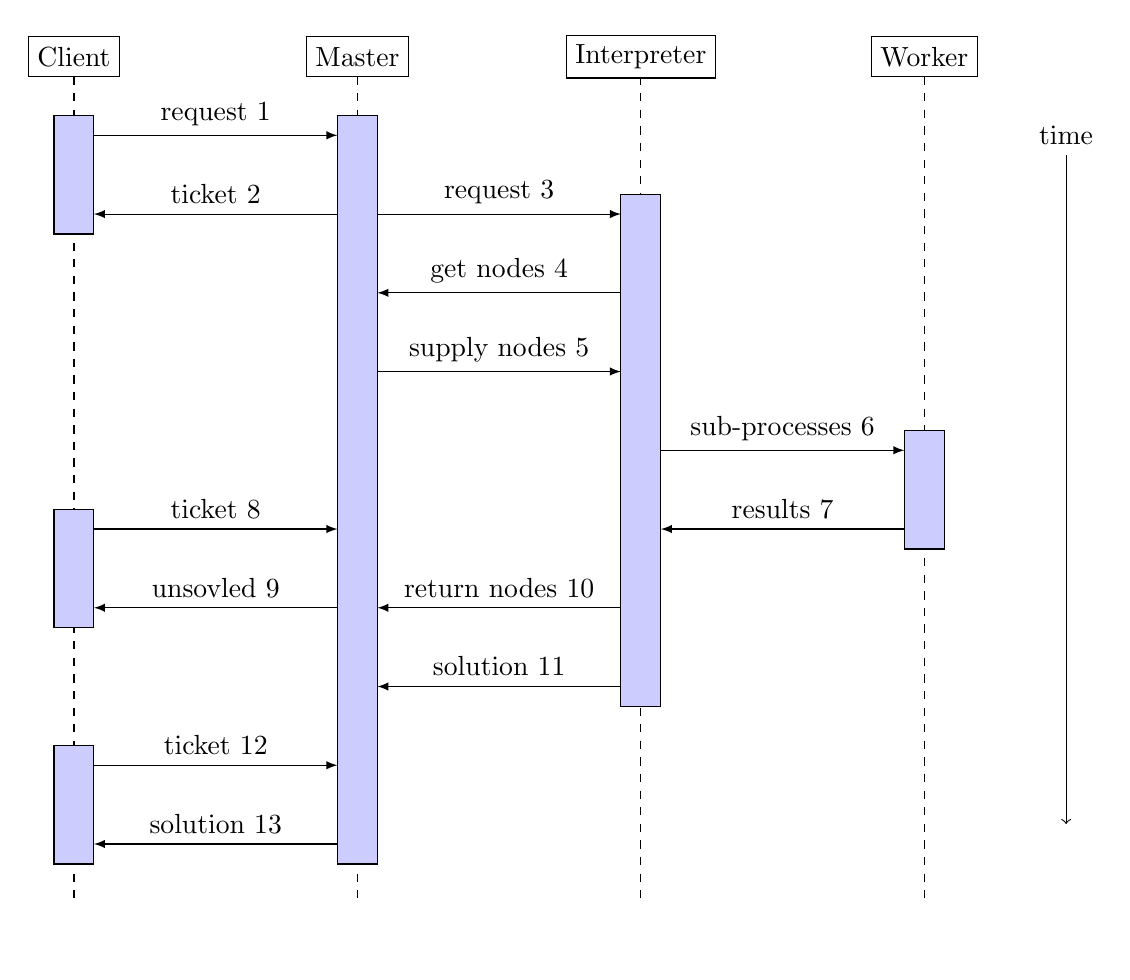
\begin{tikzpicture}[every node/.style={font=\normalsize,minimum height=0.5cm,minimum width=0.5cm},]

% Matrix
\node [matrix, very thin,column sep=1.3cm,row sep=0.5cm] (matrix) at (0,0) {
  \node(0,0) (c)  {}; &                       & \node(0,0) (m)  {}; &                       & \node(0,0) (i)  {}; &                       & \node(0,0) (ns) {}; & \\
  \node(0,0) (c0) {}; & \node(0,0) (c0m0) {}; & \node(0,0) (m0) {}; &                       &                     &                       &                     & \node(0,0) (t0) {}; \\
  \node(0,0) (c1) {}; & \node(0,0) (m1c1) {}; & \node(0,0) (m1) {}; & \node(0,0) (m1i1) {}; & \node(0,0) (i1) {}; &                       &                     & \\
  \node(0,0) (c2) {}; &                       & \node(0,0) (m2) {}; & \node(0,0) (i2m2) {}; & \node(0,0) (i2) {}; &                       &                     & \\
  \node(0,0) (c3) {}; &                       & \node(0,0) (m3) {}; & \node(0,0) (m3i3) {}; & \node(0,0) (i3) {}; &                       &                     & \\
  \node(0,0) (c4) {}; &                       & \node(0,0) (m4) {}; &                       & \node(0,0) (i4) {}; & \node(0,0) (i4n4) {}; & \node(0,0) (n4) {}; & \\
  \node(0,0) (c5) {}; & \node(0,0) (c5m5) {}; & \node(0,0) (m5) {}; &                       & \node(0,0) (i5) {}; & \node(0,0) (n5i5) {}; & \node(0,0) (n5) {}; & \\
  \node(0,0) (c6) {}; & \node(0,0) (m6c6) {}; & \node(0,0) (m6) {}; & \node(0,0) (i6m6) {}; & \node(0,0) (i6) {}; &                       &                     & \\
  \node(0,0) (c7) {}; &                       & \node(0,0) (m7) {}; & \node(0,0) (i7m7) {}; & \node(0,0) (i7) {}; &                       &                     & \\
  \node(0,0) (c8) {}; & \node(0,0) (c8m8) {}; & \node(0,0) (m8) {}; &                       & \node(0,0) (i8) {}; &                       &                     & \\
  \node(0,0) (c9) {}; & \node(0,0) (m9c9) {}; & \node(0,0) (m9) {}; &                       & \node(0,0) (i9) {}; &                       & \node(0,0) (n9) {}; & \node(0,0) (t9) {}; \\
  \node(0,0) (cx) {}; &                       & \node(0,0) (mx) {}; &                       & \node(0,0) (ix) {}; &                       & \node(0,0) (nx) {}; & \node(0,0) (tx) {}; \\
};

% Process labels
\fill 
  (c)  node[draw,fill=white] {Client}
  (m)  node[draw,fill=white] {Master}
  (i)  node[draw,fill=white] {Interpreter}
  (ns) node[draw,fill=white] {Worker}
  (t0) node                  {time};

% Vertical lifelines
\draw [dashed]
  (c)  -- (cx)
  (m)  -- (mx)
  (i)  -- (ix)
  (ns) -- (nx);

\draw [style=->] (t0) -- (t9);

% Blocks
\filldraw[fill=blue!20]
  (c0.north west) rectangle (c1.south east)
  (c5.north west) rectangle (c6.south east)
  (c8.north west) rectangle (c9.south east)
  (m0.north west) rectangle (m9.south east)
  (i1.north west) rectangle (i7.south east)
  (n4.north west) rectangle (n5.south east);

% communication
\draw [-latex] (c0) -- (m0);
\draw [-latex] (m1) -- (c1);
\draw [-latex] (m1) -- (i1);
\draw [-latex] (i2) -- (m2);
\draw [-latex] (m3) -- (i3);
\draw [-latex] (c5) -- (m5);
\draw [-latex] (i4) -- (n4);
\draw [-latex] (m6) -- (c6);
\draw [-latex] (n5) -- (i5);
\draw [-latex] (i6) -- (m6);
\draw [-latex] (i7) -- (m7);
\draw [-latex] (c8) -- (m8);
\draw [-latex] (m9) -- (c9);

\fill
  (c0m0) node[above] {request \smallfigannotation{1}}
  (m1c1) node[above] {ticket \smallfigannotation{2}}
  (m1i1) node[above] {request \smallfigannotation{3}}
  (i2m2) node[above] {get nodes \smallfigannotation{4}}
  (m3i3) node[above] {supply nodes \smallfigannotation{5}}
  (i4n4) node[above] {sub-processes \smallfigannotation{6}}
  (n5i5) node[above] {results \smallfigannotation{7}}
  (c5m5) node[above] {ticket \smallfigannotation{8}}
  (m6c6) node[above] {unsovled \smallfigannotation{9}}
  (i6m6) node[above] {return nodes \smallfigannotation{10}}
  (i7m7) node[above] {solution \smallfigannotation{11}}
  (c8m8) node[above] {ticket \smallfigannotation{12}}
  (m9c9) node[above] {solution \smallfigannotation{13}}
;
\end{tikzpicture}
  \caption{Behaviour of the system when a request is submitted by a client.}
  \label{fig:request_handling}
\end{figure}

\begin{itemize}
  \item [\figannotation{1}] The client submits a request to the master node.
  \item [\figannotation{2}] The master node replies with the assigned ticket to the client.
  \item [\figannotation{3}] The master node spawns a new process interpreter on its own node and passes the request to it.
  \item [\figannotation{4}] The interpreter asks the master node for worker nodes for the purpose of spawning processes on them.
  \item [\figannotation{5}] The master node replies with available worker nodes to the interpreter. If there are no worker nodes available, the master waits with this reply until worker nodes become available.
  \item [\figannotation{6}] The interpreter spawns processes on the worker nodes.
  \item [\figannotation{7}] Once a process on a worker node has calculated its result, it sends it back to the interpreter and terminates.
  \item [\figannotation{8}] The client supplies the previously received ticket number to the master, hoping the request has been processes completely.
  \item [\figannotation{9}] The master tells the client that its request hasn't been completely processes yet. There is no solution to the client's problem available yet.
  \item [\figannotation{10}] After execution of processes on the worker nodes, the interpreter returns them to the master node for further allocation to other interpreters. Note that steps \figannotation{4} to \figannotation{10} can, and most likely will, happen multiple times while processing a request.
  \item [\figannotation{11}] Once the interpreter has finished processing the client's request, it submits the solution to the problem to the master.
  \item [\figannotation{12}] The client supplies the ticket to the master again.
  \item [\figannotation{13}] The master responds to the client with the calculated solution.
\end{itemize}


\section{Extension for practical use}
In this chapter, we introduce an extension to the data model and process interpreter that is of relevance for practical application. The expressiveness of remains unchanged.

In the interpretation of all process combinators we pass the process' argument on to all sub-processes without altering it, all sub-processes receive the same argument. However, in some situations we might want to pass different portions of the argument to parallel sub-processes. We could achieve this behaviour by prepending some kind of projection process to each of the parallel processes: when receiving an argument it performs a projection on the value it receives and reduces it to the desired portion. In an environment where it is cheap to duplicate values, e.g. by using shared memory, this approach might be acceptable. In a situation where there is network communication involved and the same value needs to be serialised and sent to a set of remote processes though, there is potentially a high amount of communication overhead created. For this purpose, we extend our data model for processes and add two new data constructors for processes that explicitly incorporate splitting their argument and passing on \textit{different} arguments to their sub-processes. 

\subsection{Data model}
While \texttt{Parallel} is used to create a \texttt{Process} that runs two sub-processes in parallel with the same argument passed on to both of them, \texttt{Split}\index{Data constructor!Split} generalises this behaviour. It takes a function of type \texttt{a $\to$ (c, d)} and uses it to split its argument into two pieces, each of which is passed on to one of its sub-processes. The remaining arguments are analogous to the parameters of \texttt{Parallel}: two processes that should be run in parallel with types \texttt{Process c e} and \texttt{Process d f} as well as a combinator process of type \texttt{Process (e, f) b} that is used to combine the results of the sub-processes into a single value.
\begin{lstlisting}[language=Haskell,caption=Signature of the \texttt{Split} data constructor.,numbers=left,frame=bt,firstnumber=24]
Split :: (a -> (c, d))
      -> Process c e
      -> Process d f
      -> Process (e, f) b
      -> Process a b
\end{lstlisting}

The \texttt{Slice}\index{Data constructor!Slice} data constructor is a generalisation of \texttt{Split}: rather than splitting it into exactly two pieces, it takes a function of type \texttt{a $\to$ [c]} to split its input into a list of pieces. The rest of the parameters are analogous to the parameters of \texttt{Multilel}: a list of processes of type \texttt{[Process c d]}, each of which receives one slice\footnote{Given, there are equally many input slices as there are sub-processes. This potential problem motivates to do a defensive implementation for the interpretation of \texttt{Slice} processes.} of input, a value of type \texttt{b} and a combinator process of type \texttt{Process (b, [d]) b} that is used to fold the result values together. The same argument for requiring all sub-processes to be of the same type given in the discussion of \texttt{Multilel} applies.
\begin{lstlisting}[language=Haskell,caption=Signature of the \texttt{Slice} data constructor.,numbers=left,frame=bt,firstnumber=29]
Slice :: (a -> [c])
      -> [Process c d]
      -> b
      -> Process (b, [d]) b
      -> Process a b
\end{lstlisting}

\subsection{Process interpreter}
We give the implementation of the process interpreter \texttt{runProcess} for interpretation of \texttt{Split} and \texttt{Slice} processes locally in the \texttt{IO} monad. The implementation for interpretation in the \textsf{Cloud Haskell} \texttt{Process} monad is very similar again and only involves adding the necessary \texttt{master} parameter and lifting \texttt{MVar} action from the \texttt{IO} monad into the \texttt{Process} monad, it can be found in \appref{app:distributed_split_slice}.

The interpretation of \texttt{Split}\index{Process interpreter!Split} processes is very similar to the interpretation of \texttt{Parallel} processes. The only difference compared to \texttt{Parallel} is the function \texttt{split} that we use to split the argument \texttt{x} into two pieces \texttt{xl} and \texttt{xr}. We use \texttt{forkIO} to fork an instance of \texttt{runProcessHelper} and supply it with \texttt{p1}, \texttt{xl} and an empty MVar \texttt{mvar}. \texttt{runProcessHelper} runs \texttt{p1} with the argument \texttt{xl} and saves \texttt{p1}'s result in \texttt{mvar} once it terminates. When we're done running \texttt{p2} on \texttt{xr} in the interpreter thread, we obtain the value saved in \texttt{mvar}. This operation blocks until a value has been saved to \texttt{mvar}. Finally, we run \texttt{combinator} on the two result values and return its result.
\begin{lstlisting}[language=Haskell,caption=Implementation of the interpreter for \texttt{Split} processes.,label=lst:local_runprocess_multilel,numbers=left,frame=bt,firstnumber=16]
runProcess (Split split p1 p2 combinator) x = do
  let (xl, xr) = split x
  mvar <- newEmptyMVar
  _ <- forkIO $ runProcessHelper p1 xl mvar
  r2 <- runProcess p2 xr
  r1 <- takeMVar mvar
  runProcess combinator (r1, r2)
\end{lstlisting}

Interpreting a \texttt{Slice}\index{Process interpreter!Slice} process follows the same principle as interpreting a \texttt{Multilel} process. We have a list of processes \texttt{ps} that should be executed in parallel. We use the function \texttt{slice} to slice the argument \texttt{x} into slices, zip the processes \texttt{ps} together with their arguments and call them \texttt{pairs}. For each of the created pairs, we create an empty MVar so the result from running the processes on their inputs can be saved into them. Then we use \texttt{forkIO} to fork an instance of \texttt{runProcessHelper} per pair of process and argument slice and provide an MVar to save the process' result into. Finally we read the results from the MVars, automatically waiting for termination of all processes because of the blocking behaviour of MVars, and fold them together to one result using \texttt{fold} and the initial fold value \texttt{ib}.
\begin{lstlisting}[language=Haskell,caption=Implementation of the interpreter for \texttt{Slice} processes.,label=lst:local_runprocess_multilel,numbers=left,frame=bt,firstnumber=16]
runProcess (Slice slice ps ib fold) x = do
  let pairs = ps `zip` slice x
  mvars <- forM pairs (const newEmptyMVar)
  mapM_ (\((proc, x'), mvar) -> forkIO $ runProcessHelper proc x' mvar) (pairs `zip` mvars)
  ress  <- forM mvars $ \mvar -> takeMVar mvar
  runProcess fold (ib, ress)
\end{lstlisting}

Now with the \texttt{Split} process available, we can give an alternative implementation of the process interpreter for the interpretation of \texttt{Parallel} processes. Structurally and semantically, \texttt{Parallel} and \texttt{Split} are very similar, the only difference is the function that is used to split the argument into pieces in the case of \texttt{Split}. To preserve \texttt{Parallel}'s semantics, we create a function that \enquote{splits} the argument by returning a pair of the same value, and thereby duplicating it. Together with this function, we use the parameters of \texttt{Parallel} to create a \texttt{Slice} process and run \texttt{runProcess} on it.
\begin{lstlisting}[language=Haskell,caption=Alternative implementation of the interpreter for \texttt{Parallel} processes.,label=lst:local_runprocess_split,numbers=left,frame=bt,firstnumber=16]
runProcess (Parallel p1 p2 combinator) x = do
  runProcess (Split (\x -> (x,x)) p1 p2 combinator) x
\end{lstlisting}

Similarly, we can convert \texttt{Multilel} processes into \texttt{Slice} processes. Again, the semantic and structural properties are very similar, we only need to provide a function that slices the argument into the appropriate slices. Since all sub-processes from \texttt{ps} should be supplied with the argument \texttt{x}, we can simply choose \texttt{repeat} to carry out the slicing. \texttt{repeat} takes a value and returns an infinite list with each element equal to the supplied value. Together with the parameters of \texttt{Multilel}, we use \texttt{repeat} to create a \texttt{Slice} process and run \texttt{runProcess} on it.
\begin{lstlisting}[language=Haskell,caption=Alternative implementation of the interpreter for \texttt{Multilel} processes.,label=lst:local_runprocess_slice,numbers=left,frame=bt,firstnumber=16]
runProcess (Multilel ps ib fold) x = do
  runProcess (Slice repeat ps ib fold) x
\end{lstlisting}

\section{Difference to the algebraic model}
\label{chp:difference_model_implementation}
Opposed to the situation given in the algebraic model\index{Algebraic!model}, \textsc{Hive} processes are \textbf{not} pure. As mentioned in \chpref{chp:cloud_haskell}, our processes execute in the \textsf{Cloud Haskell} \texttt{Process} monad\index{Monad}, which builds on top of the \texttt{IO} monad.

For many real world applications this comes in handy. When implementing a software that solves computationally hard problems, like e.g. the travelling salesman problem\index{Traveling Salesman Problem} which will be discussed in \chpref{chp:tsp}, usually there are meta-heuristic\footnote{Meta-heuristics will be discussed in \chpref{chp:meta_heuristics}}\index{Meta-heuristic} approaches or approximation algorithms\index{Approximation algorithm} \cite{rolf2006approximationsalgorithmen} used, which make use of random number generators. Using random number generators in pure processes is not impossible, but would require to always provide a process with a seed for the random number generator.

In fact, using non-pure processes gives the developer more freedom to optimise processes manually. Instead of transmitting data structures of possibly several megabyte or even gigabyte over the network every time a process is spawned, the data could be stored in a local file on the nodes or in a database that is accessible over the network. However, this means that processes can perform operations that yield different results when executed several times, which has immediate implications for a process optimiser.

\subsubsection{Process optimiser\index{Process!optimiser}}
We have mentioned earlier that we can use the laws given in \chpref{chp:laws} to build a process optimiser that would automatically transform processes into an equivalent representation, based on defined criteria. One of such criteria might be the memory the representation of a process tree takes up or the runtime that a process will need to execute. Unfortunately it's hard to predict the runtime of a process, so the user would need to supply the optimiser with a heuristic that is capable of estimating the runtime of processes. However, based on the laws from \chpref{chp:laws} there are some situations where it seems very reasonable to optimise a composed process, such as $P \choice P$ or $P \,\parallel\, P$ for a process $P$.

But as discussed in \chpref{chp:difference_model_implementation}, a developer might make use of side-effects intentionally. He might construct a process that performs random walks in the solution space of a computationally hard problem, based on a random number generator and then run multiple instances of that process in parallel. A process optimiser would optimise this set of parallel running processes to only one process, not knowing that the processes would behave differently at runtime because they are not pure. This is why we do not provide an automated process optimiser and trust the developer to make appropriate use of the laws given in \chpref{chp:laws} whenever applicable.

\section{Example: arithmetic expressions - hello world for interpreters\index{Example}}
\label{chp:example}
After introducing the \textsc{Hive} process algebra and discussing the interpreter that takes care of the distribution of \textsc{Hive} processes, we give an example of how to make use of it. To do so, we employ the typical hello world program for interpreters, i.e. an interpreter\index{Interpreter} for arithmetic expressions\index{Arithmetic expression}. Except for imports from the \textsf{Cloud Haskell} library and the \textsc{Hive} process algebra, this example will be self-contained. It is intentionally kept very simple and the necessity for a distributed interpreter for arithmetic expressions is certainly not given. However, an interpreter for arithmetic expressions is fairly simple and thus, well suited to illustrate how to apply the \texttt{Hive} process algebra for distribution without distracting from it.

First, we need an appropriate data type to represent arithmetic expressions. An arithmetic expression \texttt{Expr} is either a value \texttt{Val} containing an \texttt{Int} or a combination of two arithmetic expressions. The combinators we want to support are addition \texttt{Add}, subtraction \texttt{Sub}, multiplication \texttt{Mul} and division \texttt{Div}. The relevant data type together with the data constructors can be found in \lstref{lst:arith_model} 
\begin{lstlisting}[language=Haskell, caption=Data model for the representation of arithmetic expressions., label=lst:arith_model, numbers=left, frame=bt]
data Expr = Val Int
          | Add Expr Expr
          | Sub Expr Expr
          | Mul Expr Expr
          | Div Expr Expr
\end{lstlisting}

When we use an interpreter to interpret an arithmetic expression, we expect it to return a value of type \texttt{Int}. The implementation of such an interpreter \texttt{eval} can be found in \lstref{lst:arith_eval} and is straightforward. The interpreted value of a \texttt{Val} expression is simply its wrapped \texttt{Int} value. The interpreted value of a more complicated expression is given by recursively interpreting the involved sub-expressions and combining the results with the appropriate operator, i.e. \texttt{+} for \texttt{Add}, \texttt{-} for \texttt{Sub}, \texttt{*} for \texttt{Mul} and \texttt{div} for \texttt{Div}.
\begin{lstlisting}[language=Haskell, caption=Implementation of an interpreter for arithmetic expressions of type \texttt{Expr}., label=lst:arith_eval, numbers=left, frame=bt, firstnumber=6]
eval :: Expr -> Int
eval (Val i) = i
eval (Add x y) = eval x + eval y
eval (Sub x y) = eval x - eval y
eval (Mul x y) = eval x * eval y
eval (Div x y) = eval x `div` eval y
\end{lstlisting}

Now, if we want to make use of the \textsc{Hive} process interpreter \texttt{runProcess} to distribute the interpretation of arithmetic expressions, we need to define a transformation from the category of arithmetic expressions \texttt{Expr} to the category of \textsc{Hive} processes \texttt{Process a b}. Arithmetic expressions of type \texttt{Expr} do not take any parameter, they are fully defined by the values incorporated into \texttt{Val} values and yield a value of type \texttt{Int} when interpreted and hence need to be mapped to \textsc{Hive} processes of type \texttt{Process () Int}.

For the representation of arithmetic expressions that have the form of \texttt{Val}, we implement a generator \texttt{val} for \textsf{Cloud Haskell} processes that are used to create basic \textsc{Hive} processes by wrapping them into a \texttt{Const} wrapper. The implementation of \texttt{val} can be found in \lstref{lst:arith_val}.
\begin{lstlisting}[language=Haskell, caption=A generator for \textsf{Cloud Haskell} process for the representation of \texttt{Val} nodes., label=lst:arith_val, numbers=left, frame=bt, firstnumber=12]
val :: Int -> CH.Process Int
val i = return i
\end{lstlisting}

Arithmetic expressions of the form \texttt{Add}, \texttt{Sub}, \texttt{Mul} and \texttt{Div} can be interpreted in parallel since their sub-expressions are independent from each other. We can exploit \texttt{Parallel} processes from the \textsc{Hive} process algebra to interpret the sub-expressions in parallel. To do so, we need to supply combinator processes for the \texttt{Parallel} processes, so the obtained results from the sub-processes can be combined into a single value. The implementation of the relevant combinator processes can be found in \lstref{lst:arith_combinators}, they all have the same type \texttt{(Int, Int) $\to$ CH.Process Int}. Remember that functions that should be wrapped into a closure need to be of arity one and return a \textsf{Cloud Haskell} process.
\begin{lstlisting}[language=Haskell, caption=\textsf{Cloud Haskell} processes for the combination of results from processes that have been executed in parallel., label=lst:arith_combinators,numbers=left, frame=bt, firstnumber=14]
add :: (Int, Int) -> CH.Process Int
add (x, y) = return (x + y)

subtract :: (Int, Int) -> CH.Process Int
subtract (x, y) = return (x - y)

multiply :: (Int, Int) -> CH.Process Int
multiply (x, y) = return (x * y)

divide :: (Int, Int) -> CH.Process Int
divide (_, 0) = undefined
divide (x, y) = return (x `div` y)
\end{lstlisting}

In addition, we need a \texttt{SerializableDict} for each type that we want to send back as a result over the network. Since the only type involved in this is \texttt{Int}, we only need a dictionary of type \texttt{SerializableDict Int}, which is shown in \lstref{lst:arith_dict}.
\begin{lstlisting}[language=Haskell, caption=\texttt{SerializableDict} for values of type \texttt{Int}., label=lst:arith_dict, numbers=left, frame=bt, firstnumber=26]
intDict :: SerializableDict Int
intDict = SerializableDict
\end{lstlisting}

Now we need to pass the list of names of all the functions that shall be able to be called remotely to the \textsf{Cloud Haskell} function \texttt{remotable}. Their names are then entered into a table of static code pointers to make the function remotely callable. They can be called on any node that shares the relevant entries in its table of static code pointers.
\begin{lstlisting}[language=Haskell, caption=Making functions remotely callable., label=lst:arith_remotable, numbers=left, frame=bt, firstnumber=28]
remotable ['val, 'add, 'subtract, 'multiply, 'divide, 'intDict]
\end{lstlisting}

To turn the previously defined functions into \textsc{Hive} processes, we need to wrap them using the type constructors for basic processes, i.e. \texttt{Const} and \texttt{Simple}. For that, we need to supply a closure\index{Closure} and a matching dictionary for the serialisation\index{Serialisation} of the result value of the respective closure per process. Since the only result type involved here is \texttt{Int}, we're fine with \texttt{SerializableDict Int}, which is created by \texttt{\$(mkStatic 'intDict)} from the previously defined \texttt{intDict} using \textsf{Template Haskell}. The dictionary itself is not sent over network and since it is a static value, i.e. it is known at compile time and doesn't need to be sent over network. It can be looked up in the table of static code pointers by its name since it has been added by supplying its top level name to \texttt{remotable}, as shown in \lstref{lst:arith_remotable}. The wrapping into \textsc{Hive} processes is shown in \lstref{lst:arith_wrapping}.
\begin{lstlisting}[language=Haskell, caption=Creating function closures and wrapping them into \textsc{Hive} processes., label=lst:arith_wrapping, numbers=left, frame=bt, firstnumber=29]
valP :: Int -> Process () Int
valP i = Const $(mkStatic 'intDict) ($(mkClosure 'val) i)

addP :: Process (Int, Int) Int
addP = Simple $(mkStatic 'intDict) $(mkClosure 'add)

subP :: Process (Int, Int) Int
subP = Simple $(mkStatic 'intDict) $(mkClosure 'subtract)

mulP :: Process (Int, Int) Int
mulP = Simple $(mkStatic 'intDict) $(mkClosure 'multiply)

divP :: Process (Int, Int) Int
divP = Simple $(mkStatic 'intDict) $(mkClosure 'divide)
\end{lstlisting}

All prerequisites are met now and we can start with the transformations from \texttt{Expr} to \textsc{Hive} processes, which we implement an interpreter for. It can be found in \lstref{lst:arith_transformation}: \texttt{interpret} maps expressions of the form \texttt{Val} to a basic process that simply returns a wrapped value and maps composed expressions to composed processes using the \texttt{Parallel} type constructor. When passing the resulting \textsc{Hive} process to the \textsc{Hive} process interpreter \texttt{runProcess}, it takes care of the distribution of the sub-processes of the \texttt{Parallel} nodes.
\begin{lstlisting}[language=Haskell, caption=Transformation from \texttt{Expr} to \textsc{Hive} processes., label=lst:arith_transformation, numbers=left, frame=bt, firstnumber=43]
interpret :: Expr -> Process () Int
interpret (Val i)   = valP i
interpret (Add x y) = Parallel (interpret x) (interpret y) addP
interpret (Sub x y) = Parallel (interpret x) (interpret y) subP
interpret (Mul x y) = Parallel (interpret x) (interpret y) mulP
interpret (Div x y) = Parallel (interpret x) (interpret y) divP
\end{lstlisting}

In this example we have defined a data structure that can be used to represent arithmetic expressions and implemented a conventional interpreter for this data structure. Then, we have defined a mapping from these arithmetic expressions to \textsc{Hive} processes, and used the \textsc{Hive} process interpreter to distribute their interpretation. We did not have to explicitly implement network communication of any kind for this, but only have to make appropriate use of the \textsc{Hive} process algebra to represent our computation as a composed process. 